\graphicspath{{pro-ndi/}}

\chapter{Learning Representative Climate-Relevant Numbers}
\label{chap:prondi}

The Numerically-Driven Inferencing (NDI) is introduced in Section~\ref{sec:ndi}.
In Chapters~\ref{chap:two} and \ref{chap:evilndi}, we have seen further
demonstrations of the kinds of marked attitudinal and conceptual shifts one can
obtain with quite minimalist interventions. In particular, we've seen the
striking effects of the EPIC procedure (both introduced by
\cite{ranney_numerically_2001_fixed}), as well as more minimal
interventions involving only the “E” (Estimate) and “I” (Inform) portions of the
EPIC intervention. (\cite{rinne_estimation_2006}, also explore the primary
importance of committing to an estimation prior to receiving the correct
information.)

As with Chapter~\ref{chap:evilndi}, we again present a collection of NDI
interventions in a somewhat different order than they were actually performed
in. This way, we are able illustrate a potential problem (the continued erosion
of confidence in one's own knowledge) that is solved in
Chapter~\ref{chap:mechanism}.  In the studies below, we presented different
participant groups with numerical information that is relevant to global climate
change acceptance.  Unlike in Chapter~\ref{chap:evilndi}, we used numbers that
were likely to boost acceptance. As before, survey methods employed in the
following studies are described in detail in Section~\ref{chap:survey}.

\section{Study 1: Online Experiment with UC Undergrads}
\label{sec:pro-uc}

Given the efficacy of “evil” numbers and previous successes of the NDI paradigm,
this study assessed the efficacy of numbers that support the claim of global
climate change. Again partly tongue-in-cheek, we call these “saintly” numbers.
Given prior NDI studies of similarly “shocking” magnitudes (e.g., Garcia de
Osuna, et al., 2004), our hypothesis was that the accurate feedback would
increase participants’ climate change acceptance, but diminish self-confidence
in their knowledge of the issue.


\subsection{Methods}

\subsubsection{Participants}

UC Berkeley undergrads ($N=60$) were recruited via the Research Participation
Pool (RPP). Prior to engaging in experiments in the RPP program, many
participants complete a pre-test screening survey containing demographics and
other items contributed by numerous experimenters. This RPP pre-test was
completed by 30 of our participants. 
% TODO: Demographics

\subsubsection{Materials and Procedure}

This study used an on-line version of materials otherwise similar to those used
in our “evil” NDI study (reported in Section~\ref{sec:evilndi-methods}), and
used a pre-test survey included in the RPP screening survey. For those
participants that completed this survey, it was completed,
on average, 18-days prior to the intervention. In the main intervention, we
queried individuals about eight quantities (listed in
Appendix~\ref{app:numbers}). The eight items were accompanied by questions
directed at participants’ surprise and their reactions to each number.
Fictitious monetary policies were left out of this version, as simple attitude
shifts were readily observed in the simplified 8-item “evil” intervention, and
these shifts are more directly comparable across experiments.  An added feature
of the online intervention is that we could remind individuals of the estimates
they gave on the same page on which they incorporated numerical feedback,
ensuring that they contrasted the two. As with online surveys in
Chapter~\ref{chap:mechanism}, an attitude and belief post-test was administered
immediately after our intervention and also after a retention interval.
% TODO: What was retention interval?


% \subsubsection{Analysis}
% 
% Analyses here were largely analagous to those described in
% Section~\ref{sec:mech-online-methods}.

\subsection{Results}

\subsubsection{Self-rated Knowledge and Surprise}

Because these items were, as anticipated and as with the “evil” items, able to
significantly erode self-rated knowledge (5.3 to 4.0, $t(29)=-3.6$, $p<0.01$).
This erosion was comparable to that found with the “evil” numbers.  The
numerical items ranked relatively high on participant surprise compared to the
(significantly effective) 400-word mechanism intervention from
Chapter~\ref{chap:mechanism}.  The mean surprise rating across items was 4.8.
While this is a bit lower than surprise ratings for “evil” numbers in
Chapter~\ref{chap:evilndi}, it markedly exceeds the mean surprise rating for the
400 words was 2.9 (all ratings above “1” indicate some level of surprise). Thus,
the immediate affective impact of these numbers was reported as \emph{higher}
than an intervention that (as we'll see in Chapter~\ref{chap:mechanism})
effectively supported significant shifts in student attitudes along with other
measures.

One of the most surprising numbers (at 5.2) was the percentage of active
researchers who support the tenets of anthropogenic climate change, reflective
of the strong relationship between perceived scientific consensus and acceptance
of climate change reported in \textcite{lewandowsky_pivotal_2013}. The two
numbers most comparable to the statistics in the 400 words were similarly
surprising, with the rises in atmospheric methane and atmospheric CO2 ranking at
5.9 and 5.1, respectively---both higher than the mean surprise ratings from the
400 words in Chapter~\ref{chap:mechanism}.


\subsubsection{GW attitutudes}

In spite of the powerful impacts described above, attitudes, acceptance, and
beliefs regarding climate change remained stable after this intervention with
“saintly” numbers (6.71 pre and 6.67 post).  This lack of effect is counter to
prior NDI studies (as well as the results reported in
Chapter~\ref{chap:mechanism}), in which individuals’ preferences and beliefs
were often markedly shifted by even a single number. 

\subsection{Discussion}


An experimental silver lining here is the demonstration that participants will
not report greater climate change acceptance merely by dint of experimenter
demand.  In both this \emph{and} previous NDI and RTMD studies, participants
were explicitly told that all feedback statistics and other information were
fully accurate, that the study involved \emph{no} deceptions.  One possible
explanation is due to a methodological change: prior studies 
also provided the particular scientific/literature source both
for each statistic that was sought and each provided as feedback.
Sources were not uniformly provided in this study. This is one
difference that may partially account for our lack-of-effect.

So, it is possible that participants were less compelled by the authority of
this study’s statistics, compared to those in Chapter~\ref{chap:evilndi}.
Another possibility is that, as in Chapter~\ref{chap:evilndi}, participants were
left feeling less knowledgeable—weakening any boost these surprising numbers
could have on climate change acceptance.  

A final possiblity is that the effect of this numerical intervention would be
strengthened by an appropriate context for integrating this information. That
is, perhaps we could not simply present our numerical information as it was in
isolation with the expectation of an effect. Indeed, as we report in
\parencite{clark_knowledge_inpress}, similar numbers had little immediate effect on
high-school students as a part of a global warming mechanism curriculum.
However, students exposed to numbers like those in this study retained the
effects of the curriculum to a greater extent than students in a control
condition.

A possibility that will disconfirmed in the introduction to the following
section is that this lack of result was due to the delay between attitudes
assessed during during RPP prescreening and our core intervention. As we'll
shortly see, this lack-of-result was replicated within a single session
intervention.

\section{Study 2: Online intervention with Amazon Mechanical Turk}
\label{sec:pro-mturk}

After the difficulty obtaining shifts in GW attitudes and beliefs above, I was
able to replicate this difficulty by presenting the same materials to a more
general population on Amazon Mechanical Turk. I won't go through the
exercise of reporting another null result here, apart from mentioning that
unlike the above, this intervention contained a full “sandwich” in a single
survey/session. Thus, it seems unlikely that our difficulty in observing a
result with these particular materials depends on the timing of the pretest.

I then engaged in a thorough examination of the wording of the items (also
discovering that one item was off by an order of magnitude). This process was
relatively informal, and consisted of showing the items to naïve individuals and
asking them if they had any difficulty understanding them. Descriptions were
iterated until they appeared to make sense to non-experts.

\subsection{Methods}

\subsubsection{Participants}
\label{sec:CCO-ndi-participants}

“Workers” on the Amazon Mechanical Turk platform ($N=40$) were recruited to
complete a two-part survey. Language used in recruitment made no mention of
climate change, and was titled “Politics, Numbers, and Your Attitudes.” After
removal of problematic participants above, we were left with 38 participants in
the intervention. 18 of the total retained participants were female. One
participant reported being born outside the United States, but residing here for
20 years. Stated party affiliations are listed in
Table~\ref{table:cco-mech-party}. Mean conservativism was 4.0 ($sd=2.1$).
Compared with our college students above, conservativism was in the same
ballpark and participants were far more likely to declare Democrat or Republican
than with our college students above. While the sample is still clearly biased
towards the Democratic/liberal end of the political spectrum, the ratio
between Republicans and Democrats is far less extreme than previous samples. 

% latex table generated in R 2.15.1 by xtable 1.7-1 package
% Fri Jun 21 16:05:32 2013
\begin{table}[ht]
\centering
\begin{tabular}{rcc}
  \toprule
      & party (percentage) \\ 
  \midrule
  democrat &  17 (44.7) \\ 
  independent &  12 (31.5) \\ 
  republican &   4 (10.5) \\ 
  libertarian &   3 (7.8) \\ 
  other &   1 (2.6) \\ 
  decline to state &   1 (2.6) \\ 
  \midrule
  total &  38 (100.0) \\ 
   \bottomrule
\end{tabular}
\end{table}

% This is a spurious result, as our own demographics didn't separate protestants
% and catholics
% A final interesting feature of our population is that all participants reporting
% their faith as Christian self-identified as Catholic. That is, we had no
% “protestant” participants.

\subsubsection{Materials and Procedure}

Materials are largely identical with those in Study 1, apart from the
improvements in comprehensibility described above. An additional improvement in
terms of making the survey more clear was replacing a fill-in-the-blank question
for specifying units and “increase” or “decrease” for their estimate. In this
version of the experiment, one or two choices including the unit and direction
were provided as appropriate to each estimate. For example, “\% of researchers”
or “feet increase.” The item reproduced in Appendix~\ref{app:format-ndi} is an
exact copy of the format used for this study.  Note that participants were
further asked to indicate their experience of an item on three different
scales---one asking about “surprise,” one about “embarrassment at lack of
knowledge,” and one about the novelty vs familiarity of the item.

Note that in the process of streamlining instructions, I removed instructions to
the effect that \emph{no} deceptions were used. This is in contrast to the previous
(ineffective) study that did include such an instruction.  In addition, in this
study even more than in the above study, the inclusion of information about
authority was scant (e.g., the more accessible phrase “journal article” replaced
phrases such as “article published in PNAS”). The exact wording used in this
study is shown in Appendix~\ref{app:numbers}.

A final change was the removal of an item on sea-level rise which had previously
been incorrectly reported as 10 times higher than the true amount. It is a small
possibility that this item undermined individual's belief in our other numbers,
but based on comments, only a few individuals appeared to doubt the number.

\subsubsection{Data quality on Amazon Mechanical Turk}
\label{sec:mturk-problems}

The use of an anonymous, on-line labor pool raises concerns about data quality.
For example, people may try to take the survey again or they may lie about their
demographics (i.e., claiming they are U.S. residents so that they may gain the
credit). Re-taking is one of the most easily guarded against concerns on Amazon
Mechanical Turk, as Amazon will attempt to enforce this if requested, as was
done in this study. However, in addition, no IP addresses were repeated in the
participant for this study.

Amazon will attempt to restrict individuals to the U.S. if requested, and this
was done for this experiment. An additional layer of verification of location is
straightforward using “geo IP” databases. In this case, geographical locations
were retrieved using the GeoLite data created by MaxMind (available from
\url{http://www.maxmind.com}). On our survey, participants indicated the state
they reside in. Participant IP addresses were subsequently checked against this
reported location. Here, two individuals IP’s appeared to be located in Germany
and Guatemala, and thus these participants were excluded. Most other
participants had IP addresses that resolved to the state they claimed to be
from. One participant’s IP address was not listed in the MaxMind database, and
was traced to either Hughes Net or Bright Home, both U.S.-only satellite
internet providers.

\subsection{Results}

\subsubsection{Surprise and related measures}

Numbers were again ranked as surprising, and in a similar range to that observed
in the above Study (which failed to shift attitudes). Here, we have a total of
21 measures of something like surprise, 3 for each of our 7 estimation items.
The number of potential relationships is large here, so we must be cautious in
over-interpreting \emph{post hoc} observation. However, some clear structure
appears to exist amongst these correlations, as can be seen in
Figure~\ref{fig:CCO-prondi-surp-corr}. Specifically, based on the block
structure near the diagonal for the “embarrassment” and familiarity ratings, it
seems that individuals had a tendency to rate these items relatively low or high
across items, while “surprise” provided a relatively item-pure measure. This can
be summarized statistically with the averages of the off-diagonal correlations
in these blocks. The surprise items had a mean correlation with each other of
0.14, while the embarrassment and familiarity items had a mean of 0.41 and 0.40,
respectively. Another clear structure can be seen in the smaller diagonals
visible off the main diagonal. Where these diagonals appear, this indicates that
for a given item, the relevant measures tended to covary. The mean of the
correlations along these minor diagonals were as follows: surprised with
embarrassed was 0.57, surprised with familiar was -0.31, and embarrassed with
familiar was -0.09. Thus, embarrassment and familiarity do a poor job of
predicting one another. Surprise, however, is well correlated with the
embarrassment rating, and still reasonably correlated with familiarity.

\begin{figure}
    \centering
    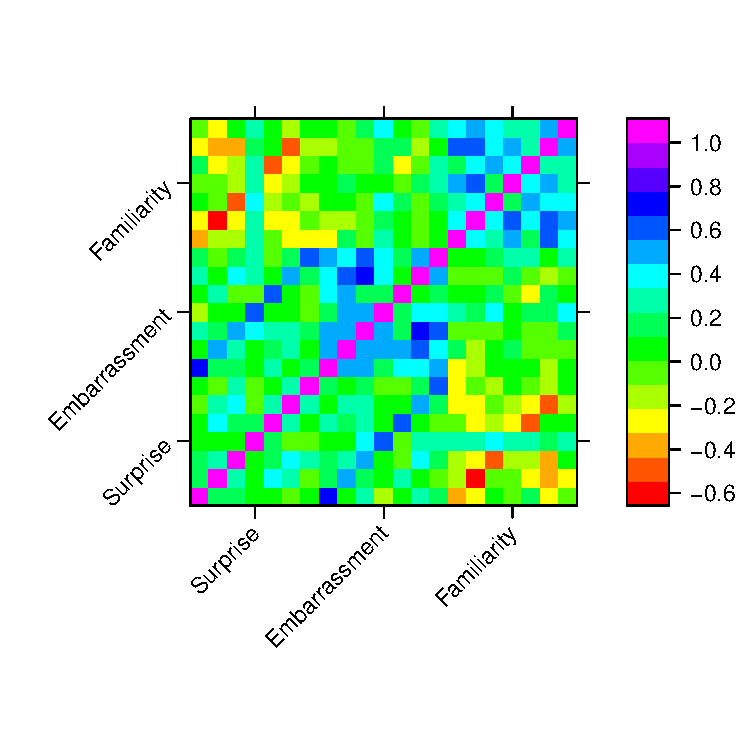
\includegraphics{CCO-prondi-surp-corr.pdf}
    \caption{An image plot of the correlations between ratings for each of the 3
        ratings across the 7 estimation items. Each rating type is presented in
        a block (textual labels apply to items within the entire block).
        Relatively clear block structure is apparent surrounding the main
        diagonal for embarrassment and familiarity (here, indicated by blue for
        higher values). Parallel to the main diagonal, a blue / high correlation
        diagonal of positive correlations can be seen within an item between
        embarrassment and surprise, and a red / negative correlation diagonal
        can be seen for surprise and familiarity.}
    \label{fig:CCO-prondi-surp-corr}
\end{figure}

Across items, surprise ranged from 3.2 to 6.3, embarrassment from 2.6 to 4.3,
and familiarity from 2.9 to 4.1. Some floor effects may have occurred for
embarrassment and familiarity (the opposite of what we'll see in
Chapter~\ref{chap:mechanism}. The order of items was consistent across
surprise and embarrassment (but not for familiarity). 

Overall, it appears that our surprise question is the most pure assessment of
student response to the item, and for these numbers, it suffers from less of a
floor effect. That said, no combination of mean or maximum surprise (and
related) scores were significantly predictive of shifts in GW belief and
concern.

\subsubsection{GW acceptance supported by clear numerical information}

This version of the intervention did significantly boost mean GW acceptance and
concern by about 1/3 of a point, as depicted in Figure~\ref{fig:prondi-gw}. The
shift was significant ($t(37) = 2.74$, $p < 0.01$). Thus, it appears that while
we (and others) experience some failures of numeracy to achieve shifts in the
direction of scientific consensus, it appears that a carefully crafted
intervention can have useful effects.

\begin{figure}
    \centering
    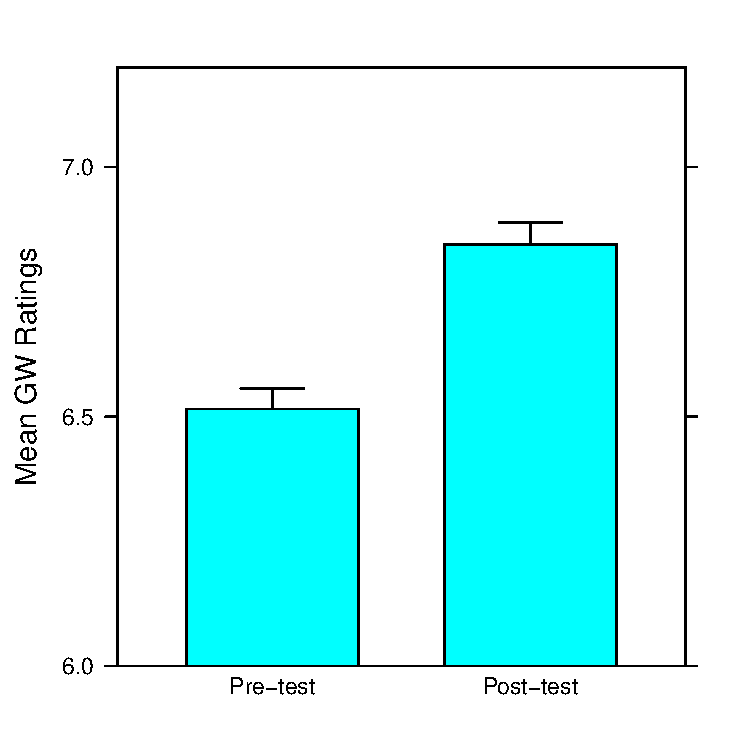
\includegraphics{CCO-prondi-gw.pdf}
    \caption{Shifts in GW ratings in Mechanical Turk intervention with
        climate-change-supporting numbers.}
    \label{fig:prondi-gw}
\end{figure}

\subsubsection{Self-confidence in GW knowledge is still eroded}

While we see shifts above towards the scientific consensus on global warming,
participants still report feeling 0.97 points less knowledgeable as depicted in
Figure~\ref{fig:prondi-knw}. This drop is significant ($t(37)=-3.38$, $p<0.001$).

\begin{figure}
    \centering
    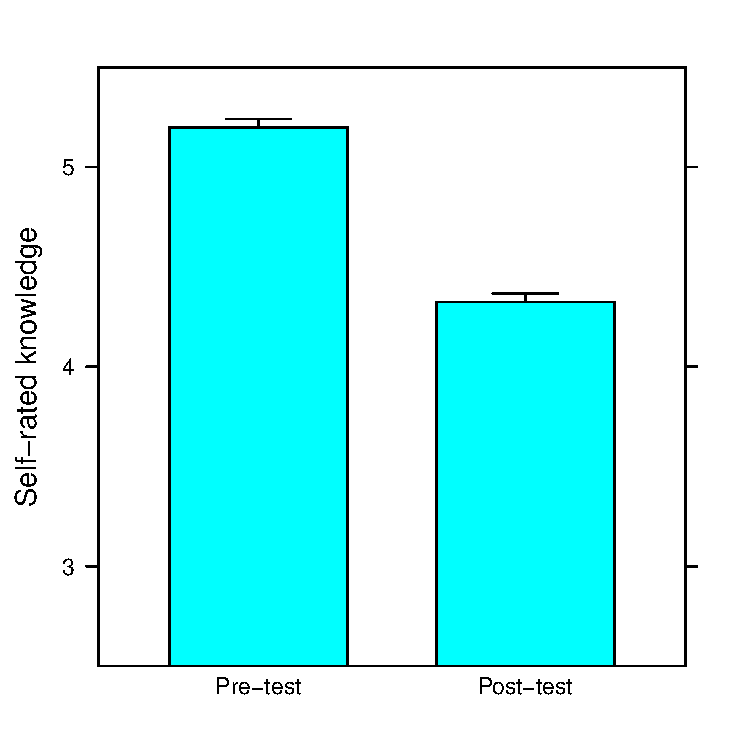
\includegraphics{CCO-prondi-knw.pdf}
    \caption{Erosion of confidence in self-ratings of GW knowledge in Mechanical
        Turk intervention with climate-change-supporting numbers.}
    \label{fig:prondi-knw}
\end{figure}

% \subsubsection{No observed effect of political variables}
% 
% TODO?
% With this sample, we are able to examine the effects of
% conservativism or political party. Figure XXX shows attitudes broken out by
% Republican, Democrat (and Other).

\subsection{Discussion}

As compared with Study 1, the primary change was an increase in the fluency of
materials. While we should be careful in making comparisons across populations,
the similarity in the effects reported in Chapter~\ref{chap:mechanism} provide
some evidence that similar interventions perform similarly across UC Berkeley
undergrads and Mechanical Turkers. Thus, it seems reasonable to recommend that
careful attention be given to materials like those used in this chapter. Items
should be tested for comprehensibility with naïve individuals prior to
attempting to use them in a belief or behavioral change intervention.

Note also that for reasons of time and simplicity, we did not include policy
shifts in this study. However, we can still compare the size of belief and
attitude shifts with the 2-item study described in Chapter~\ref{chap:evilndi}
and infer that we are seeing attitudinal shifts of a similar magnitude.

\section{Summary and Conclusions}

Despite the “failure” of Study 1 above, it affords us a number of insights.
Critically, we cannot simply throw a set of numbers at Americans and expect that
to impact their beliefs and attitudes. A real silver lining here is support for
the conclusion that shifts, when we do observe them, are \emph{not} driven
merely by experimenter demand. While we cannot claim to know for sure what “went
wrong” with Study 1, there are a few notable differences.  In both studies, not
all items had sources, but sources were further simplified (and sometimes
omitted) in Study 2. Many were likely difficult to understand in Study 1
(wordings in Appendix~\ref{app:numbers} are reflective of the final wordings
used in Study 2). Unlike Study 2, Study 1 \emph{did} include the assertion that
the study involved no deceptions. Thus, the most obvious explanation is that a
certain degree of comprehensibility is necessary to effect shifts in GW
attitudes and beliefs, but proper experimentation is necessary to come to a firm
conclusion.

Combined with Chapter~\ref{chap:evilndi}, we have now witnessed numeracy-based
interventions that push individuals towards and away from the scientific
consensus on anthropogenic climate change. In addition, we have seen that even
when students claim surprise regarding a set of numbers, they may not be
influenced by these numbers unless they are presented with the necessary clarity.

It should be noted also that as in Chapter~\ref{chap:evilndi}, participants were
left feeling less knowledgeable than they reported prior to the intervention. It
remains for future research to determine what impact this might have on
behavior, but it seems likely that a lack of confidence would likely
inhibit public statements or commitments regarding climate change.

Our group has also integrated such numbers with  more comprehensive
interventions. For example, \textcite{clark_knowledge_inpress} reports on the
utility of such numbers in improving retention of a climate change curriculum
described in \textcite{felipe_numerical_2012}. In the following chapter, we'll
see another relatively simple, but more comprehensive intervention that includes two
of our more surprising numbers. This intervention leaves participants both more informed
\emph{and} more confident in their own knowledge.

\section*{Acknowledgements}

The work reported in this chapter has been previously published, in part, in
\textcite{clark_knowledge_inpress}.  All such material is re-used here with the
permission of my co-authors, the publishers, and the Graduate Division at the
University of California, Berkeley.
